\chapter{Related Works}\label{chapter:related_works}

This chapter presents a literature review focusing especially on work with public mission sensors, and is organized as follows: section \autoref{sec:rreview} presents previous surveys and reviews relevant to the work. Section \ref{sec:taxonomy} proposes a taxonomy to categorize applications in the area, and the following sections detail such applications, such as Parcel Delineation (\autoref{sec:parcel_segmentation}), Crop Mapping (\autoref{sec:crop_mapping}), Crop Yielding (\autoref{sec:crop_yielding}), LULC (\autoref{sec:lulc}), and Change Detection (\autoref{sec:change_detection}). Finally, \autoref{sec:rdiscussion} presents a critical discussion of the state of the art, identifying gaps in the literature.

\section{Reviews}\label{sec:rreview}

Some systematic reviews have been conducted covering aspects of agricultural \ac{RS} using machine learning. \fromsurvey{As an example, the work conducted by \cite{yuan2020deep} serves as introductory material for the use of \ac{DL} focusing on environmental applications. In contrast, \cite{ma2019deep} cover both urban and agricultural \ac{RS}, though their focus is on urban applications. The most referenced application is \ac{LULC}, with almost twice as many papers as second place, Object Detection. Data Fusion only appears in fifth place. As the most common architecture, \acs{CNN}s are the architecture of choice in this domain, being five times more used than \ac{AE}. The use and good results with \ac{HR} and \ac{VHR} images continued. However, there are a few multi-temporal methodologies cited that are useful in agriculture.  Also, due to its release date, this review does not cover the current rapid growth of attention-based architectures in agricultural \ac{RS} applications, including Transformers and Data Fusion applications.}

\fromsurvey{Another review was conducted by \cite{li2022deep} that studied multimodal Data Fusion in \ac{RS} considering 598 papers, from 2015 to 2022, focusing on tasks like classification (i.e. segmentation), cloud removal, and object detection. The research incorporated multiple data types such as medium and high-resolution imagery, \ac{LiDAR}, and \ac{SAR} data. They identified \acs{CNN}s as the predominant models. Despite a notable rise in publications about this subject, the authors highlighted a deficiency of datasets specifically for agricultural uses in their study. Additionally, they mentioned an issue with the interpretability and validity of synthetic data produced through Data Fusion.}

\fromsurvey{\cite{aleissaee2023transformers} mapped the use of \acs{ViT}s in \ac{RS} using 60 papers. Primarily, high-resolution multispectral imagery was used, sometimes in combination with \ac{SAR} data. The majority of papers cited in this work refer to either classification or detection problems. The survey also noted that pretraining using \ac{RS} data instead of natural images - in most cases, ImageNet Dataset \citep{deng2009imagenet} - tends to provide better outcomes. Nevertheless, this survey did not include unsupervised pretraining, i.e., \ac{SSL}; the authors noted the absence of large-scale datasets for unsupervised pretraining. Additionally, techniques applied to \ac{SITS} were not charted in this study.}

\fromsurvey{As noted in previous efforts \citep{liu2024diffusion}, following the trend of traditional computer vision literature, \ac{RS} researchers have started to adopt diffusion models, especially since 2023. In addition, the authors argue that satellite imagery presents some noise: optical imagery presents atmospheric dispersion of \ac{EMR}, which is usually improved by so-called atmospheric corrections models \citep{li2018amosphericcorrection}; on the other hand, \ac{SAR} data has speckle inherent due to the out-of-phase reflection of \ac{EMR} from the target \citep{dasari2015sarspeckle}.For this reason, diffusion models tend to perform well because they learn latent representations that are robust to noise due to diffusion. Although the first applications were for data synthesis (i.e., Super Resolution and Cloud Removal), there are already applications for image interpretation. The authors did not specifically address agricultural applications.}

\fromsurvey{When it comes to applications, \cite{joshi2023remote} reviewed Crop Mapping and Yield in 81 selected papers. Unlike the abovementioned surveys, the authors stated that low and medium resolution optical imagery was most frequently used. Sentinel-1 MSI/Sentinel-2 data are usually used for crop mapping, while the most commonly used satellite for crop yield is \ac{MODIS}. As for \ac{DL} architectures, the most widely used model is \ac{CNN}, with more than twice the number of uses of second place, \ac{RNN}. U-Net stands out in \ac{CNN}, especially U-Net 3D for considering time series. Moreover, attention mechanisms are frequently incorporated into these architectural frameworks. Concerning the challenges identified, the authors noted a deficiency of datasets, which hinders the development of models capable of generalizing effectively. Furthermore, there is a lack of research dedicated to the interpretability of predictions.}

\fromsurvey{Both \cite{weiss2020remote} and \cite{joshi2023remote} present more recent reviews of the \ac{RS} literature, though with little information on automating image understanding using \ac{DL} and ML in general. Multiple studies indicate that crop mapping with optical data combined with \ac{SAR} leads to better results. For crop yielding, combining satellite data with \textit{in-situ} data, soil, and climate information is often an effective approach.}

\fromsurvey{Most recently, \cite{kamilaris2018deep} published the latest survey on \ac{DL} in agricultural \ac{RS}, in 2018. Authors noted that the use of \ac{DL} for \ac{RS} can generate better outcomes, hence being an alternative for shallow learning. The authors pointed out that, even today, there is a limited number of publicly available agricultural \ac{RS} datasets. Nonetheless, due to its publication date, methodologies such as \ac{SSL} were not presented in this survey.}

\fromsurvey{Also, in a more specific direction, \cite{sishodia2020applications}, reviewed the main Precision Farming methods. The survey highlighted the importance of this \ac{RS} technique for increasing agricultural productivity while minimizing environmental and social impacts. However, the review does not provide much information regarding \ac{DL} though it emphasized the method was likely to become increasingly important in meeting this challenge.}

\fromsurvey{\cite{9875399} made an extensive survey of Self-Supervised Learning methods applied to the context of urban and agricultural \ac{RS} in 2022. Traditional methods that utilize red, green, and blue (RGB) images inspired techniques for analyzing multi- and hyperspectral satellite images; similar approaches for time series were also influenced by these methods. In contrast, there are no experimental analyses for agricultural datasets. The only application tested in this work was \ac{LULC}, which is shown to be less effective for agricultural studies compared to other applications. In addition, due to its publication date, only studies up to 2021 were analyzed, and, as shown in Section \ref{sec:taxonomy}, the area has advanced significantly using modern techniques better adapted to \ac{RS} and agricultural \ac{RS}.}

\fromsurvey{\cite{begue2018remote} presented a similar review, focusing on \ac{RS} for mapping cropping practices. The authors categorize applications into crop succession, cropping patterns, and crop management techniques. However, the survey uses data from both public and commercial missions. Furthermore, due to the publication date, the survey does not include techniques such as attention models and \ac{SSL}.}

\fromsurvey{Finally, \cite{weiss2020remote} present a meta-review of the main surveys in the area of \ac{RS} for agriculture. Their study considered research up to 2019, although they did not mention the number of studied reviews. The study also includes the use of machine learning techniques on satellite data, as well as on \ac{UAV} and \ac{LiDAR}, despite not presenting a direct comparison between their results. The paper provides a summary of the typical data types employed in various applications.}

\section{Taxonomy}
\label{sec:taxonomy}

Regarding our fine-grained review, we researched papers for all useful applications in an agricultural monitoring pipeline using \ac{RS}, with a greater focus on \ac{DL} and Self-Supervised Learning. It should be noted that some papers outside the query were added due to their importance to the field. \fromsurvey{We found 905 articles on this topic, 2 of which were published under the same name in different journals. Most are from Scopus, ACM, IEEE and arXiv journals, using the FindPapers algorithm \citep{grosman2020findpapers}, considering papers from $1^{st}$ January 2019 to $2^{nd}$ December 2024. We emphasize that we only selected papers that use optical and radar images from satellites. \ac{UAV} and \ac{LiDAR} sensors on board UAVs or satellites were not considered, as there are differences in spatial resolution and data processing, which would lead to difficulties in comparing the different techniques.}

\fromsurvey{The query used for selecting papers is as follows:}

\begin{quote}
	Query = ``([\textsc{deep learning}] OR [\textsc{DL}] OR [\textsc{self-supervised}] OR [\textsc{self-supervised learning}] OR [\textsc{SSL}] OR [\textsc{MoCo}] OR [\textsc{SeCo}] OR [\textsc{SimSiam}] OR [\textsc{VicregL}] OR [\textsc{DINO}] OR [\textsc{BYOL}] OR [\textsc{Masked Auto Encoder}] OR [\textsc{SWaV}] OR [\textsc{SimCLR}]) AND ([\textsc{crop}] OR [\textsc{land cover}] OR [\textsc{change detection}] OR [\textsc{deforestation}] OR [\textsc{agriculture}]) ND NOT ([\textsc{survey}] OR [\textsc{review}]) AND NOT ([\textsc{urban}]) AND ([\textsc{remote sensing}]) AND NOT ([\textsc{lidar}] OR [\textsc{uav}])''
\end{quote}

\fromsurvey{To visualize our results, we show in Figure \ref{fig:tax_publishedpapers} a diagram of publications per publisher, which shows that the vast majority of publications in this area were published by Scopus, followed by IEEE. In addition, the number of publications per year is shown in Figure \ref{fig:tax_papersperyear}. The increase in published papers between 2023 and 2024 is evident and can be attributed to several factors, one of which is the accessibility of cloud computing. In addition, we have conducted an analysis of the frequency with which these approaches have been used over time (see Figure \ref{fig:tax_approaches_years}).}

\begin{figure}[htbp]
	\centering
	\caption{\fromsurvey{Diagram for papers and their publishers.}}
	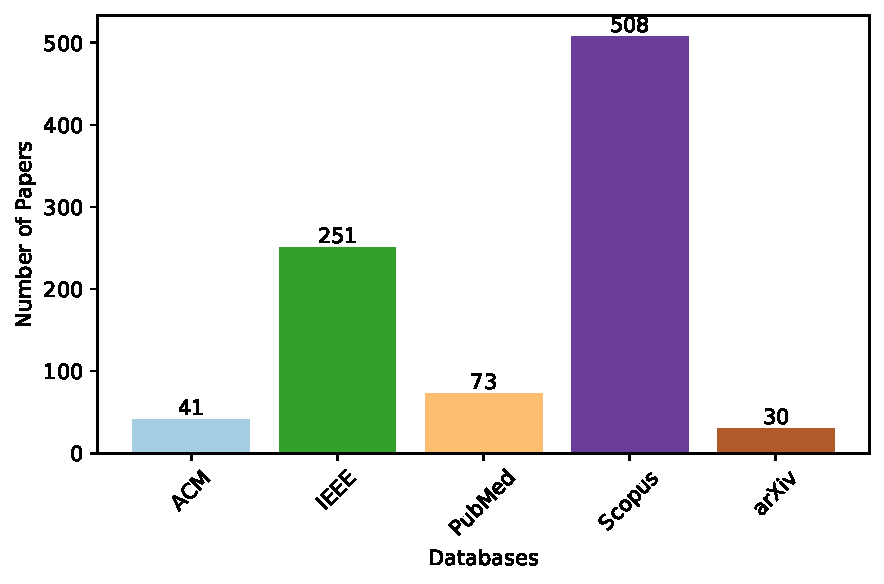
\includegraphics[width=.85\linewidth]{figures/4_related_works/taxonomy/count_published_papers.pdf}
	\label{fig:tax_publishedpapers}
\end{figure}


\begin{figure}[htbp]
	\centering
	\caption{\fromsurvey{Number of published papers per year.}}
	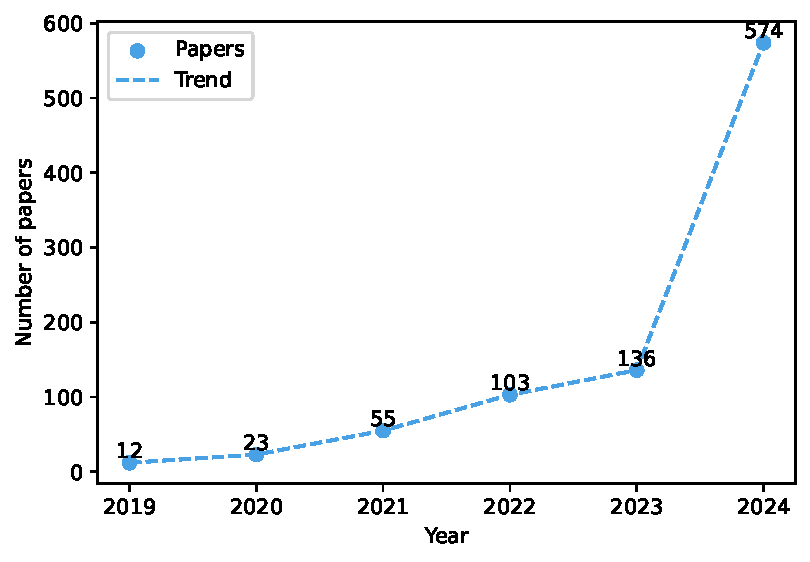
\includegraphics[width=.85\linewidth]{figures/4_related_works/taxonomy/papers_per_year.pdf}
	\label{fig:tax_papersperyear}
\end{figure}


\begin{figure}[htbp]
	\centering
	\caption{\fromsurvey{Cumulative approach of used approaches over the years.}}
	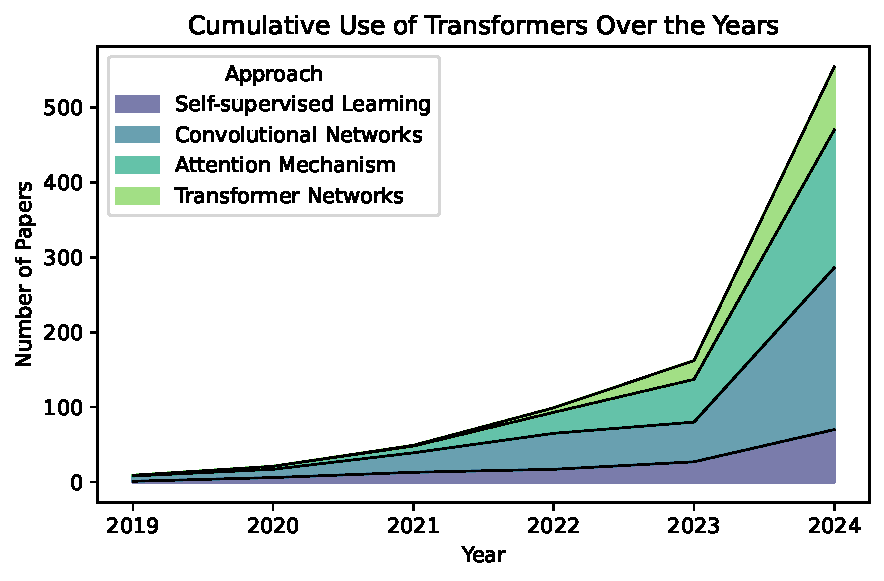
\includegraphics[width=.85\linewidth]{figures/4_related_works/taxonomy/cumulative_approaches.pdf}
	\label{fig:tax_approaches_years}
\end{figure}


\fromsurvey{As far as applications in agriculture are concerned, 503 of the 903 works referred to agriculture, i.e. $\approx. 56\%$ of all works found. To analyze their application, we created the Venn diagram in Figure \ref{fig:tax_vennapp}, which shows how frequently they are used in these 503 articles. The diagram shows that the documents related to crop mapping clearly outnumber the documents for the second most common application, change detection. The other applications appear to have been used relatively evenly for \ac{DL} research over the last five years.}

\begin{figure}[htbp]
	\centering
	\caption{\fromsurvey{Venn diagram for applications for selected papers.}}
	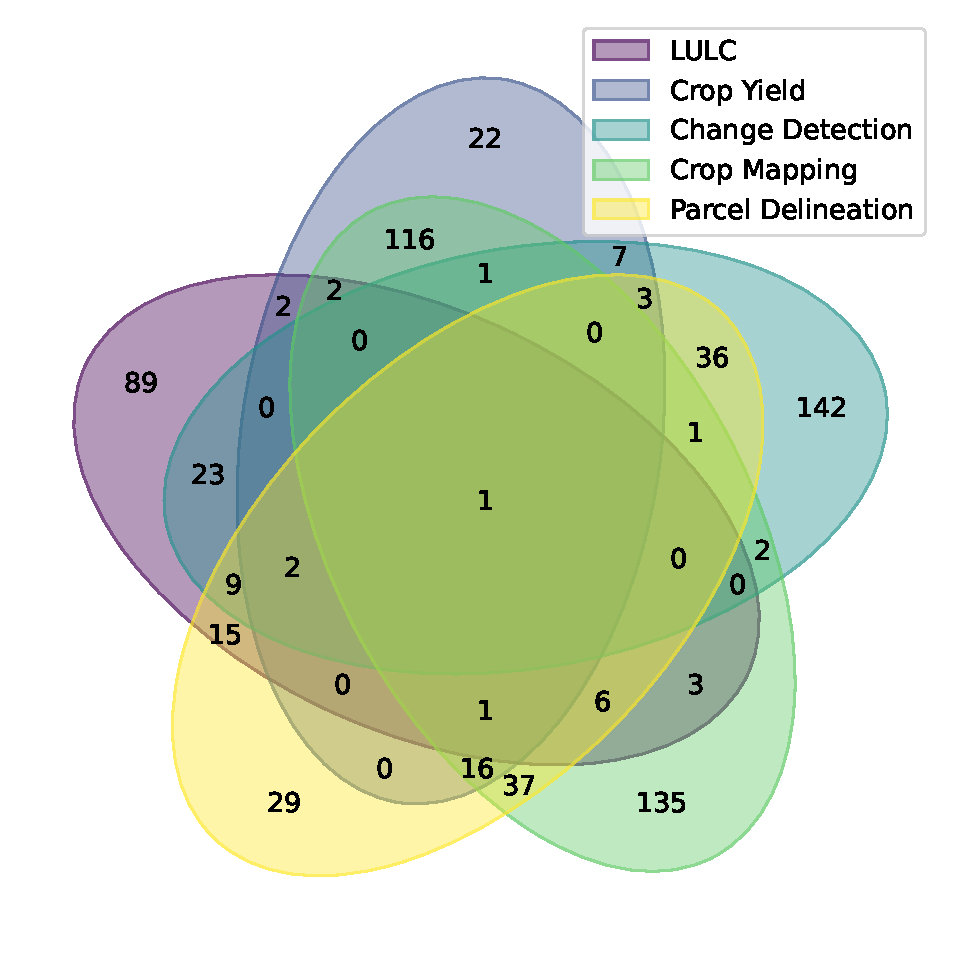
\includegraphics[width=.7\linewidth]{figures/4_related_works/taxonomy/venn_diagram_application.pdf}
	\label{fig:tax_vennapp}
\end{figure}

\fromsurvey{According to the results in Figure \ref{fig:tax_vennapp}, there are only a few overlaps between the selected topics: \ac{LULC}, Crop Yield, Change Detection, Crop Mapping, and Parcel Delineation. Although all these segments of agricultural \ac{RS} are studied separately, for some reason, they are not studied together. \ac{LULC} studies usually show agricultural classes and these studies also show forests, which together with Change Detection, can help in monitoring deforestation, such as PRODES in Brazil \citep{Almeida2022PRODES}. As for the other segments, Crop Yield, Crop Mapping, and Parcel Delineation, complement each other to form a complete and comprehensive study of \ac{RS} for agriculture \citep{sishodia2020applications}.}

\setcitestyle{super}
\begin{figure*}[!ht]
    \centering
    \caption{Proposed taxonomy for Deep Learning Remote Sensing related works.}
    \begin{tikzpicture}[
        tax_node/.style={rectangle, draw=gray!60, fill=gray!15, very thick, minimum size=5mm},align=center]
        
        \node (pic) at (0, 0) {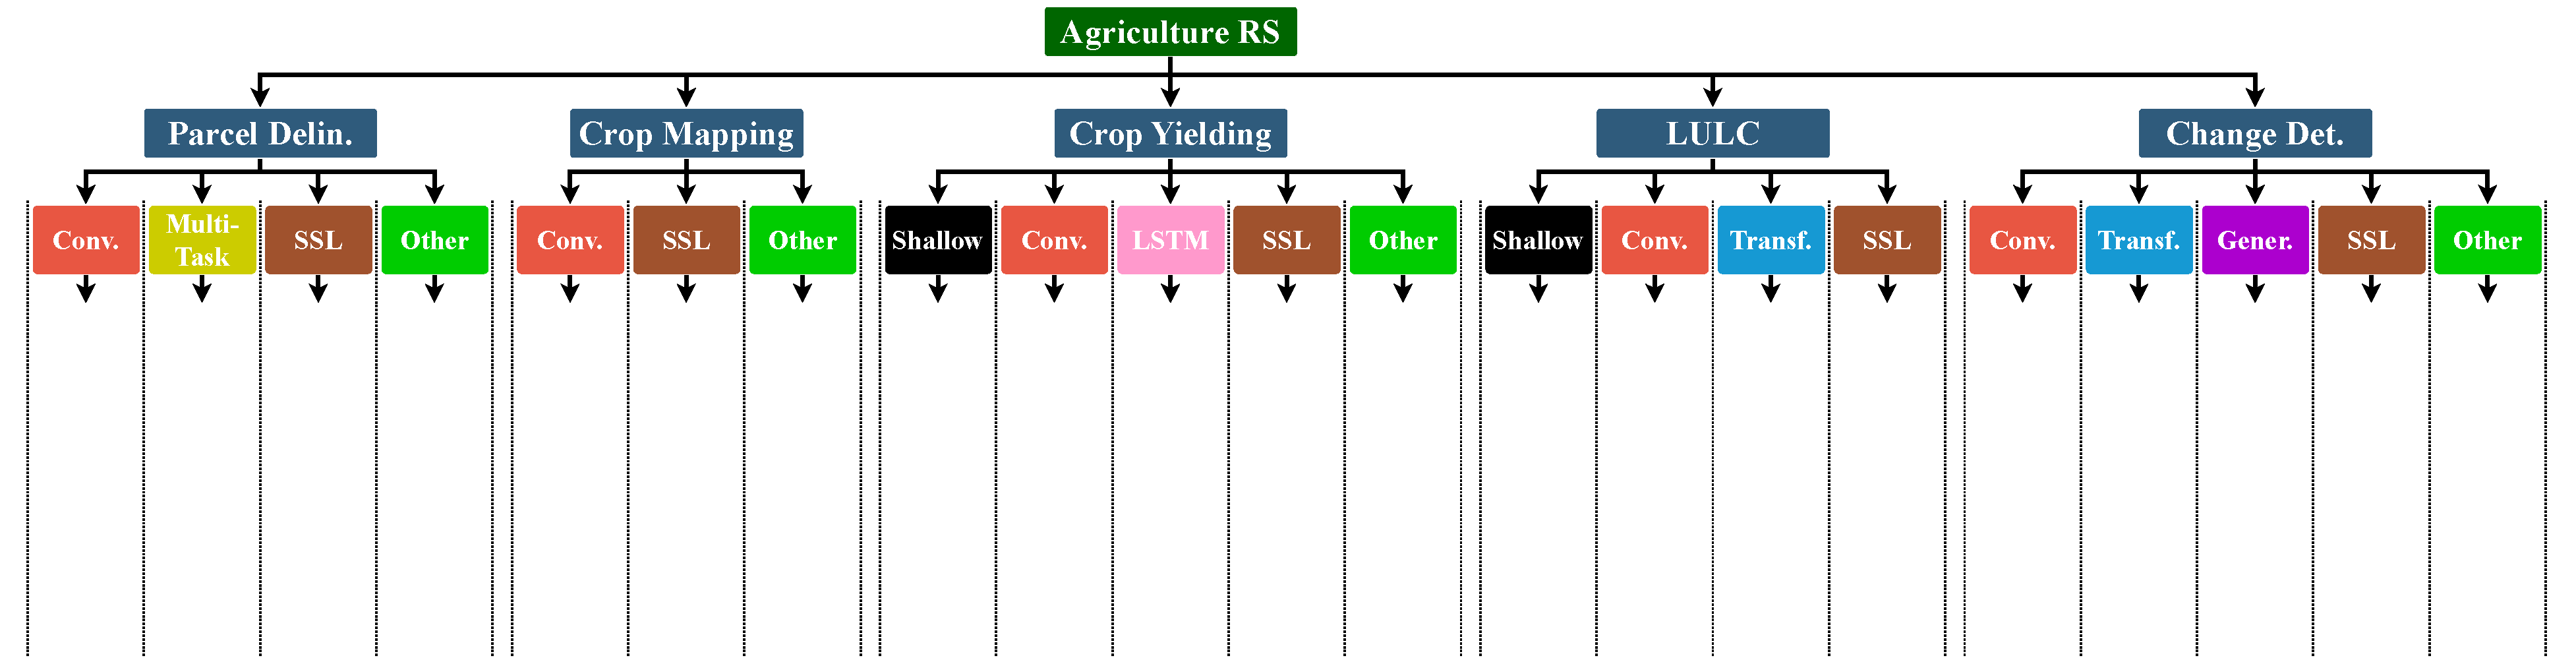
\includegraphics[clip,trim=0in -1in 0in 0in,width=\currprop]{figures/4_related_works/taxonomy/taxonomy.pdf}};
        
        %%%%%%%%%%%%%%%%%%%%%%%%%%%%%%%%%%%%%%%%%%%%%%%%%
        %%%%%%%%%%%%%%%%%%%%%%%%%%%%%%%%%%%%%%%%%%%%%%%%%
        % Parcel Segmentation.
        
        \node (parcel_conv1) at (\wparcelconv, \hfir) 
        {\refsize \cite{xu2022delineation}};
        \node (parcel_conv2) at (\wparcelconv, \hsec) 
        {\refsize \cite{xie2023edge}};
        \node (parcel_conv3) at (\wparcelconv, \hthi) 
        {\refsize \cite{zhang2023novel}};
        \node (parcel_conv4) at (\wparcelconv, \hfou) 
        {\refsize \cite{waldner2020deep}};
        
        \node (parcel_mt1) at (\wparcelmt, \hfir) 
        {\refsize \cite{li2023using}};
        \node (parcel_mt2) at (\wparcelmt, \hsec) 
        {\refsize \cite{yan2024tsanet}};
        \node (parcel_mt3) at (\wparcelmt, \hthi) 
        {\refsize \cite{10664585}};
        \node (parcel_mt4) at (\wparcelmt, \hfou) 
        {\refsize \cite{zhao2023fastsegment}};
        \node (parcel_mt5) at (\wparcelmt, \hfif) 
        {\refsize \cite{10644049}};
        
        \node (parcel_ssl1) at (\wparcelssl, \hfir) 
        {\refsize \cite{calhoun2022self}};
        
        \node (parcel_other1) at (\wparcelother, \hfir) 
        {\refsize \cite{huang2022unsupervised}};
        \node (parcel_other2) at (\wparcelother, \hsec) 
        {\refsize \cite{osco2023segment}};
        \node (parcel_other3) at (\wparcelother, \hthi) 
        {\refsize \cite{kerner2024multi}};

        %%%%%%%%%%%%%%%%%%%%%%%%%%%%%%%%%%%%%%%%%%%%%%%%%
        %%%%%%%%%%%%%%%%%%%%%%%%%%%%%%%%%%%%%%%%%%%%%%%%%
        % Crop Mapping.
        
        \node (mapping_conv1) at (\wmappingconv, \hfir) 
        {\refsize \cite{yaramasu2020pre}};
        \node (mapping_conv2) at (\wmappingconv, \hsec) 
        {\refsize \cite{xu2020deepcropmapping}};
        \node (mapping_conv3) at (\wmappingconv, \hthi) 
        {\refsize \cite{gallo2021sentinel}};
        \node (mapping_conv4) at (\wmappingconv, \hfou) 
        {\refsize \cite{farmonov2023crop}};
        \node (mapping_conv5) at (\wmappingconv, \hfif) 
        {\refsize \cite{gallo2022in_season}};
        
        \node (mapping_ssl1) at (\wmappingssl, \hfir) 
        {\refsize \cite{yuan2020self}};
        \node (mapping_ssl2) at (\wmappingssl, \hsec) 
        {\refsize \cite{yuan2022sits}};
        \node (mapping_ssl3) at (\wmappingssl, \hthi)
        {\refsize \cite{xu2024self}};

        \node (mapping_other1) at (\wmappingother, \hfir)
        {\refsize \cite{XU2021112599}};
        \node (mapping_other2) at (\wmappingother, \hsec) 
        {\refsize \cite{mena2023comparative}};
        \node (mapping_other3) at (\wmappingother, \hthi) 
        {\refsize \cite{abbas2023towards}};
        \node (mapping_other4) at (\wmappingother, \hfou) 
        {\refsize \cite{russwurm2023end}};
        \node (mapping_other5) at (\wmappingother, \hfif) 
        {\refsize \cite{mirzaei2023enhancing}};
        
        %%%%%%%%%%%%%%%%%%%%%%%%%%%%%%%%%%%%%%%%%%%%%%%%%
        %%%%%%%%%%%%%%%%%%%%%%%%%%%%%%%%%%%%%%%%%%%%%%%%%
        % Crop Yielding.
        
        \node (yielding_shallow1) at (\wyieldshallow, \hfir) 
        {\refsize \cite{huber2022extreme}};
        \node (yielding_shallow2) at (\wyieldshallow, \hsec) 
        {\refsize \cite{cheng2022wheat}};
        \node (yielding_shallow3) at (\wyieldshallow, \hthi) 
        {\refsize \cite{sabo2023deeper}};
        \node (yielding_shallow4) at (\wyieldshallow, \hfou) 
        {\refsize \cite{goel2024crop}};
        
        \node (yielding_conv1) at (\wyieldconv, \hfir) 
        {\refsize \cite{lu2024goa}};
        \node (yielding_conv2) at (\wyieldconv, \hsec) 
        {\refsize \cite{huber2024leveraging}};
        
        \node (yielding_lstm1) at (\wyieldlstm, \hfir) 
        {\refsize \cite{gavahi2021deepyield}};
        \node (yielding_lstm2) at (\wyieldlstm, \hsec) 
        {\refsize \cite{jeong2022predicting}};
        \node (yielding_lstm3) at (\wyieldlstm, \hthi) 
        {\refsize \cite{lang2023integrating}};
        
        \node (yielding_ssl1) at (\wyieldssl, \hfir) 
        {\refsize \cite{lin2023mmst}};
        
        \node (yielding_other1) at (\wyieldother, \hfir) 
        {\refsize \cite{ma2021multi}};
        \node (yielding_other2) at (\wyieldother, \hsec) 
        {\refsize \cite{liu2022rice}};
        \node (yielding_other3) at (\wyieldother, \hthi) 
        {\refsize \cite{ilyas2023automated}};
        
        %%%%%%%%%%%%%%%%%%%%%%%%%%%%%%%%%%%%%%%%%%%%%%%%%
        %%%%%%%%%%%%%%%%%%%%%%%%%%%%%%%%%%%%%%%%%%%%%%%%%
        % LULC.
        
        \node (lulc_shallow1) at (\wlulcshallow, \hfir) 
        {\refsize \cite{abdi2020land}};
        \node (lulc_shallow2) at (\wlulcshallow, \hsec) 
        {\refsize \cite{dou2024large}};
        
        \node (lulc_conv1) at (\wlulcconv, \hfir) 
        {\refsize \cite{CNN_sun2021supervised}};
        \node (lulc_conv2) at (\wlulcconv, \hsec) 
        {\refsize \cite{CNN_xu2022land}};
        \node (lulc_conv3) at (\wlulcconv, \hthi) 
        {\refsize \cite{CNN_zhan2023multi}};
        \node (lulc_conv4) at (\wlulcconv, \hfou) 
        {\refsize \cite{CNN_zhao2022cnn}};
        \node (lulc_conv5) at (\wlulcconv, \hfif) 
        {\refsize \cite{AT_zhu2021spectral}};
        \node (lulc_conv6) at (\wlulcconv, \hsix) 
        {\refsize \cite{farmonov2023crop}};
        \node (lulc_conv7) at (\wlulcconv, \hsev) 
        {\refsize \cite{AT_zheng2022rotation}};
        
        \node (lulc_transf1) at (\wlulctransf, \hfir) 
        {\refsize \cite{TRAN_sun2022spectral}};
        \node (lulc_transf2) at (\wlulctransf, \hsec) 
        {\refsize \cite{yao2023extended}};
        
        \node (lulc_ssl1) at (\wlulcssl, \hfir) 
        {\refsize \cite{tarasiou2022embeddingearthselfsupervisedcontrastive}};
        \node (lulc_ssl2) at (\wlulcssl, \hsec) 
        {\refsize \cite{moore2023selfsupervisedapproachlandcover}};
        \node (lulc_ssl3) at (\wlulcssl, \hthi) 
        {\refsize \cite{calhoun2022self}};
        \node (lulc_ssl4) at (\wlulcssl, \hfou) 
        {\refsize \cite{moore2023selfsupervisedapproachlandcover}};
        \node (lulc_ssl5) at (\wlulcssl, \hfif) 
        {\refsize \cite{XUE2025110959}};

        %%%%%%%%%%%%%%%%%%%%%%%%%%%%%%%%%%%%%%%%%%%%%%%%%
        %%%%%%%%%%%%%%%%%%%%%%%%%%%%%%%%%%%%%%%%%%%%%%%%%
        % Change Detection.
        
        \node (change_conv1) at (\wchangeconv, \hfir) 
        {\refsize \cite{gao2019change}};
        \node (change_conv2) at (\wchangeconv, \hsec) 
        {\refsize \cite{li2021combined}};
        \node (change_conv3) at (\wchangeconv, \hthi) 
        {\refsize \cite{song2022csanet}};
        \node (change_conv4) at (\wchangeconv, \hfou) 
        {\refsize \cite{ye2023adjacent}};
        \node (change_conv5) at (\wchangeconv, \hfif) 
        {\refsize \cite{miao2023snunet3+}};
        \node (change_conv6) at (\wchangeconv, \hsix) 
        {\refsize \cite{huang2023smads}};
        
        \node (change_transf1) at (\wchangetransf, \hfir) 
        {\refsize \cite{chen2021remote}};
        \node (change_transf2) at (\wchangetransf, \hsec) 
        {\refsize \cite{yan2023transy}};
        \node (change_transf3) at (\wchangetransf, \hthi) 
        {\refsize \cite{shafique2023ssvit}};
        \node (change_transf4) at (\wchangetransf, \hfou) 
        {\refsize \cite{zhang2023multi}};
        \node (change_transf5) at (\wchangetransf, \hfif) 
        {\refsize \cite{tang2024siamese}};
        \node (change_transf6) at (\wchangetransf, \hsix) 
        {\refsize \cite{chen2024visiontwinnet}};
        
        \node (change_gen1) at (\wchangegen, \hfir) 
        {\refsize \cite{du2019unsupervised}};
        \node (change_gen2) at (\wchangegen, \hsec) 
        {\refsize \cite{tang2021unsupervised}};
        
        \node (change_ssl1) at (\wchangessl, \hfir) 
        {\refsize \cite{tao2023tov}};
        \node (change_ssl2) at (\wchangessl, \hsec) 
        {\refsize \cite{feng2024feature}};
        
        \node (change_other1) at (\wchangeother, \hfir) 
        {\refsize \cite{10460113}};
        \node (change_other2) at (\wchangeother, \hsec) 
        {\refsize \cite{hou2019w}};
        \node (change_other3) at (\wchangeother, \hthi) 
        {\refsize \cite{du2023concatenated}};
        \node (change_other4) at (\wchangeother, \hfou) 
        {\refsize \cite{zhao2023triple}};
        \node (change_other5) at (\wchangeother, \hfif) 
        {\refsize \cite{bandara2024ddpmcddenoisingdiffusionprobabilistic}};
        \node (change_other6) at (\wchangeother, \hsix) 
        {\refsize \cite{wen2024gcdddpmgenerativechangedetection}};
        \node (change_other7) at (\wchangeother, \hsev) 
        {\refsize \cite{jia2024siamesemeetsdiffusionnetwork}};
        
    \end{tikzpicture}
    \fromsurvey{Classification of the selected articles under the proposed categories of the taxonomy presented in this work. Each category can be further divided into more refined groups according to the methods' characteristics. Each method may fall under more than one group, as they are not mutually exclusive.}
    \label{fig:taxonomy_paper_alocation}
\end{figure*}

\setcitestyle{authoryear, round}


\section{Parcel Delineation}
\label{sec:parcel_segmentation}

\fromsurvey{Parcel delineation, also known as cropland delineation, is the application that separates a given region into agricultural plots. This application operates on an image or time series of images (i.e. sequence of images), aiming to output a list of polygons that circumvent agricultural tiles. In addition, the application can be seen as semantic segmentation \citep{xu2022delineation}, instance segmentation, or object detection \citep{osco2023segment}. In this sense, several traditional metrics can be used to determine the output quality, such as \ac{OA}, \ac{IoU}, \ac{mAP} and \ac{mAR}. However, agricultural plots can be quite irregular, which means that such metrics do not represent the quality of model predictions very well, since they were designed for Bounding Boxes. For this purpose, the GTC error metric \citep{LONG2022102871} based on object detection was developed, which considers the over- and underclassified areas, weighing them according to the areas of each plot.}

\fromsurvey{Recently, the \Acf{SAM} was introduced and adapted to the \ac{RS} context \citep{osco2023segment}. Preliminary tests using \ac{VHR} and \ac{UAV} imagery demonstrated its potential. However, it has not been tested on \ac{LR}, \ac{MR}, or \ac{HR} images, and all the datasets evaluated by the authors were derived from \ac{UAV} sensors. The authors also highlighted the need for auxiliary inputs, such as text or bounding boxes, refining the predictions, and recommending further investigation of the model's applicability to \ac{RS}. It is important to note that, using \ac{SAM}, the \ac{SAM} UKFields project generated a dataset of agricultural plots (see Table \ref{tab:context_labeled_datasets}) for the regions of England, Wales, Scotland, and Northern Ireland using harmonic terms from MSI/Sentinel-2 \ac{NDVI} time series, regardless of the quality of this parcel delimitation has not been qualified.}

\fromsurvey{Authors generally used \acs{CNN}s or variations to delineate agricultural parcels. \cite{xu2022delineation} used a U-Net with separable depth-wise convolution layers called DSCUnet to raw segment and classify agricultural areas, then, a Richer Convolutional Features Network was employed to refine the boundary delineation of the parcels from agricultural classified regions obtained by the former step, using single \ac{VHR} images from the Gaofen-2 satellite. The authors pointed to misclassification issues when the study area contains small buildings close to agricultural parcels. \cite{xie2023edge} propose the High-Resolution Network (HRNet), a \ac{CNN} integrated with an attention module that retains feature information at different scales via parallel multiresolution branches. These branches are merged and fed into two modules: (i) an object-contextual module, which enhances the representation of contextual information and outputs parcel edge results, and (ii) a connectivity attention module, designed to extract connection and directional information. The outputted parcels are post-processed to merge erroneously oversegmented plots. Similarly, \cite{zhang2023novel} utilized DeepLabV3 on \ac{VHR} imagery, integrating public maps with \ac{MR} MSI/Sentinel-2 time series, to detect agricultural geometries using sequences of \ac{NDVI} values. Another notable contribution in this context is the work of Waldner and Diakogiannis \citep{waldner2020deep}, who proposed a \ac{DL} approach to extract field boundaries using a modified U-Net architecture known as Fractal ResUNet. The method was designed to operate efficiently on medium-resolution satellite data such as Sentinel-2, combining convolutional layers with residual and fractal blocks to improve boundary detection in large-scale agricultural landscapes.}

\fromsurvey{However, there is a tradeoff in these methods: the better the classification of the boundaries between the plots, the smaller the plots become when compared to the labels. The closer the plots are to the original areas, the thinner their boundaries with their neighbors, and the greater the chances of merging plots incorrectly. Siamese/multi-stream architectures are a growing trend in parcel delineation to balance this tradeoff. \cite{li2023using} used a two-branched convolutional Semantic Edge-Aware multi-task Neural network (SEANet) architecture: the first branch was responsible for drawing parcels, and the second one was to fine-delimit their boundaries. The two pieces of information were combined using a multitask loss formed by a Binary Cross-Entropy and a Dice Loss to deal with class imbalance and training instability. The method was tested for single-image segmentation using Gaofen-2 and Sentinel-2 satellite imageries. \cite{yan2024tsanet} also used a dual-stream architecture with each branch using the same idea as the former paper but with \ac{SITS} as input and weighting joining the same losses instead of a simple sum, which allows choosing between better pixel-level metrics or more consistent parcels. This approach is very similar to Two-Stream Attention Network (TSANet), and both were tested in the same study region (close to the entire area of the Netherlands) with MSI/Sentinel-2, although on different datasets, achieving similar results. \cite{10664585} advanced the technique and used the frozen decoder of a simplified version of the Foundation Model called Fast\acs{SAM} \citep{zhao2023fastsegment} as the decoder of a multi-branch architecture named Two-Flow Network (TFNet), achieving a 0.6\% \ac{OA} improvement and 0.025\% GTC error reduction on the same SEANet dataset, showing that a hybrid model can work. Finally, \cite{10644049} did similar research, developing the Boundary-Field Interaction Network (BFINet) strategy but using a Pyramid Vision Transformer as a pretrained decoder in ImageNet, as well as adding modules to refine spatial details in high-level features and merge multiscale semantic information, specially designed to deal with small and irregular plots, achieving a 0.11\% improvement in \ac{OA} and 0.95\% GTC error reduction compared to SEANet, but on another dataset than the one originally used, which prevents direct comparison with TFNet.}

\fromsurvey{At last, \cite{kerner2024multi} showed that datasets do not generalize well to different regions and present that the possibility of simple Transfer Learning of a dataset from one geographic area or satellite sensor to a different target dataset may improve the metrics in the target dataset. The authors showed that this approach works best for datasets with little labeled data by improving up to 6\% the achieved F1-Score. There are also some different strategies,  \cite{huang2022unsupervised} employed an unsupervised parcel delineation using a Convolutional Graph Neural Network adapting the traditional Graph-based Unsupervised Superpixel-Aggregation method, balancing a loss function that considers both spatial and spectral affinities, generating better results than other unsupervised techniques generating results with MSI/Sentinel-2 for regions of China.}

Some self-supervised learning contrastive (see Section \ref{sec:ssl_contrastive}) methods were used as pretraining for Parcel Delineation models. Calhoun et al. \citep{calhoun2022self} showed that SwAV pretraining, first conducted on ImageNet and then with continued pretraining on \ac{RS} data, demonstrated that Transfer Learning performed in this way yields better results than the traditional approach. However, several tasks were analyzed by the authors, and the task that showed the least improvement was precisely Parcel Delineation, with only a 0.07 increase in \ac{IoU}. Furthermore, it was observed that the larger the labeled dataset, the smaller the impact of \ac{SSL} pretraining.

\fromsurvey{Finally, according to \cite{xie2023edge}, \acs{CNN}s seem to have reached their limit in this task, and researchers have begun testing new architectures. Both \cite{li2023using} and \cite{yan2024tsanet} proposed examples of the most prominent architecture focusing on dual stream and/or multitasking and removing noise from non-existent plots. The literature reports several available datasets for parcel delineation, although \cite{kerner2024multi} claims there is little geographical variety to these areas. Further, foundational models like \ac{SAM} show innovation potential but require additional research to adapt them for broader \ac{RS} applications beyond \ac{VHR} imagery.} Regarding the use of \ac{SSL} pre-training, there is very little work in this area, and only minimal improvements have been reported.

\ac{SAM}-based approaches continue to evolve, addressing limitations in zero-shot generalization for agricultural applications. \cite{xie2025fabsamfarmlandboundarydelineation} proposed fabSAM, a hybrid framework combining a Deeplabv3+-based prompter with a fine-tuned \ac{SAM} decoder. This method achieved significant improvements over zero-shot \ac{SAM}, surpassing it by 23.47\% in \ac{mIoU} on the AI4Boundaries dataset by effectively generating mask and point prompts from intermediate segmentation outputs. Concurrently, \cite{lavreniuk2025delineateflowfastcountrylevel} introduced Delineate Anything (DelAny), an instance segmentation model based on YOLOv11 and trained on the massive FBIS-22M dataset (22.9 million field instances). DelAny demonstrated superior zero-shot performance across diverse agro-ecological zones, achieving over 100\% higher \ac{mAP} and 400$\times$ faster inference compared to SAM2. This resolution-agnostic approach reformulates delineation as instance segmentation to prevent field merging, enabling the generation of topologically consistent national-scale maps.

\section{Crop Mapping}
\label{sec:crop_mapping}

\fromsurvey{Crop mapping is the application in which, given a parcel or a map, a classification per parcel or pixel is generated for certain crops, usually using a time series of \ac{RS} images. Datasets from a given region may not generalize well to other areas due to climatic or agricultural calendar differences \citep{gadiraju2023remote}. Crop mapping is usually divided between (i) post-harvest, with the season already complete, and (ii) in-season classification, also called early prediction.}

\subsection{Post-harvest classification}

\fromsurvey{Post-harvest classification is the sub-application of Crop Mapping in which the result is obtained after the harvest, i.e. with all available agricultural time series data. This sub-application is more common in the literature, as it is simpler due to the greater amount of data available.}

\fromsurvey{CNNs are one of the most used strategies for Crop Mapping, as in \cite{gallo2021sentinel} that used a 3D \ac{CNN} Features Pyramid Network to classify \ac{SITS} crops pixel-wise using multispectral images from MSI/Sentinel-2, using a CELoss to construct the Crop Parcels and an MSELoss to determine in which time interval it is more probable to be Crop Season. Integrating attention mechanisms in a \ac{CNN} is the strategy adopted by \cite{farmonov2023crop} to extract long-term features and classify crops at the pixel level, achieving 97.89\% of \ac{OA} with hyperspectral images. The method proposed by \cite{yaramasu2020pre} used a bidirectional Long Short-Term Memory (LSTM) with a convolutional structure for generating embeddings as a temporal encoder with a pretrained ImageNet Very Deep Convolutional Networks (VGG), specifically in its VGG11  version\footnote{In VGG11, 11 stands for the total number of weight layers: 8 convolutional and 3 fully connected- used.} as a spatial encoder to predict crop mapping using crop rotation from previous years with Landsat \ac{SITS} as training.}

SSL pre-training was also employed in the application of Crop Mapping, especially in Transformer and post-Transformer models. \fromsurvey{MIM strategies were used. \ac{SITS}-\ac{BERT} \citep{yuan2020self} leverage generative pretraining for \ac{BERT} models via masking a pixel \ac{SITS} with high-value pixels to simulate clouds and training the network for reconstructing it. \ac{SITS}-\ac{BERT} proposes a modification of the transformer's positional encoder to incorporate the \ac{DoY} in order to integrate information from the agricultural calendar. Like all other \ac{SSL} methods, the pretraining is followed by fine-tuning to incorporate semantic information about crop types. \cite{yuan2022sits} further refined their strategy by using a convolutional transformer architecture to handle time series of 5x5 patches. The pretraining followed the same methodology, seeking to reconstruct the central pixel of each patch. The results were slightly better than the predecessor model, achieving an improvement of approximately 1.7\% in \ac{OA}.}

\fromsurvey{There are also contrastive \ac{SSL} models in Crop Mapping that pretrain transformer backbones. Xu et al. \citep{xu2024self} used them for Post-harvest Crop Classification, creating the model \ac{SITS}-MoCo, in which the band values are used as input series in the transformer, while the \ac{DoY} is used as input order for Positional Encoding, in addition to \ac{NDVI} Seq2Vec as pooling to reduce dimensionality in the time series to use the information in the classification head. As pretraining, MoCo was used, wherein multiple domain-specific augmentations were employed, including removal of random bands, random band switches, displacement of the time series, and changes in timestamp values, among others. The authors states that the model achieves state-of-the-art performance, even when compared to modern Masked Image Modeling methods \citep{yuan2020self,yuan2022sits}.} More recently, building upon the of \ac{SITS}-\ac{BERT}, \cite{shravan2024sits} introduced \ac{SITS}-BERT++, incorporating a dual activation function strategy, utilizing Swish for the overall model architecture to improve gradient flow, while retaining GeLU for the classification \ac{MLP}. Additionally, temporal data augmentations were also used. Also, a multihead attention mechanism was used in the top of the model in the pre-training reconstruction stage. These enhancements resulted in an improvement of nearly 3\% \ac{OA}    on the California dataset compaired to the original \ac{SITS}-\ac{BERT} \citep{yuan2020self}.

\subsection{In-season classification}

\fromsurvey{In-season classification is the sub-application of crop mapping that produces the result before the harvest. It is usually desirable to correctly classify crops as early as possible, given the economic advantages, especially with the reduced use of satellite images, which provides a cost reduction. It is a more complex application than post-harvest classification, as there is less data available.}

\fromsurvey{Several approaches focus on early recognition using \acs{CNN}s and recurrent models, as \cite{gallo2022in_season} that utilized a 3D \ac{CNN} to classify parcels over time, enabling early-season predictions. \cite{yaramasu2020pre} employed a bidirectional ConvLSTM for in-season crop mapping. \cite{xu2020deepcropmapping} developed an \ac{LSTM} capable of making predictions both during and after the season, with minimal performance differences between early and late predictions.}

\fromsurvey{\cite{russwurm2023end} presented a classification head that can be attached to any \ac{SITS} crop mapping model, allowing for in-season crop mapping. This classification head outputs the probability of the classification being correct given the number of timestamps compared to the full season, trained with an Earliness-Rewarded Loss, turning the model into a multimodal approach. The methodology was tested with an \ac{LSTM} model, being able to predict the Crops using from 16\% to 40\% of the \ac{SITS}.}

\subsection{Mixed strategies}

\fromsurvey{It is worth mentioning some other mixed strategies also researched. For example, \cite{abbas2023towards} proposed a temporal encoder capable of learning a crop mapping representation from a given region, then retrained in another area with a different agricultural calendar, done by transformers PE output computed on the source region is used as a proxy to quantify the temporal shift concerning the PE output obtained on the target region.}

\fromsurvey{An extensive analysis of the interpretability of Crop Mapping models presented by \cite{xu2024new} showed that the most significant band for crop differentiation is usually \acs{SWIR}1 ($\approx$ 1600nm). Additionally, the authors claim that, when trained with the entire season, the last timestamps are mostly widely used for prediction rather than early parts of the season. \cite{XU2021112599} proposed a Bayesian Active Learning Network capable of identifying which samples have to be labeled to represent a greater increase in information from the dataset, which can help reduce high labeling costs.}

\fromsurvey{\cite{yang2022ppce} designed a new loss function called Phenological Prior Cross Entropy (PPCE) based on traditional \ac{CELoss}, which weights probabilities based on \ac{NDYI} to capture the common yellowness of the flowering period of crops and on \ac{NDVI} for the senescence period. It prioritizes the correction of misclassified pixels based on phenological likelihood. }

\fromsurvey{\cite{mena2023comparative} tested the fusion of optical and \ac{SAR} data, as well as climatological data for Crop Mapping. It was reported that the fusion of these data types improves classification, especially with feature-level fusion using gates, resulting in a 0.34\% improvement in accuracy on the tested datasets. \cite{mirzaei2023enhancing} also employed Data Fusion, but only between \ac{SAR} and optical data; they created tabular features and used a Conditional Adversarial Generative Network (CTGAN) to generate synthetic data of the most underrepresented classes.}

\section{Crop Yielding}
\label{sec:crop_yielding}

\fromsurvey{Crop yield prediction is a regression application that typically uses the geometry of a crop region and the growth cycle dates to forecast production. Several methods combine satellite images with other sources of information, such as weather data and soil information. It is a difficult application to generalize, and there is little amount of datasets for it, which means that Shallow Learning is still used in addition to \ac{DL} techniques, as stated by \cite{goel2024crop}. Moreover, methodologies are rarely directly compared, as many datasets are private. Therefore, various techniques are used to address the issue of limited data volume.}

\fromsurvey{Shallow learning methods are still widely used. \cite{huber2022extreme} compared two \ac{DL} methodologies, \ac{CNN} and \ac{CNN} \ac{LSTM}, with the Shallow Learning XGBoost methodology for soybean crop yield, concluding that the traditional method performed better. However, the authors also claimed that larger datasets can improve the metrics of \ac{DL} techniques. \cite{sabo2023deeper} compared shallow and \ac{DL} methods, concluding that traditional ones performed better in their experiments due to the small size of the available dataset for barley, durum, and soft wheat crop yielding. \cite{cheng2022wheat} also compared the traditional techniques, Random Forest, Gradient Boosting Decision Tree, used in the XGBoost framework, and \ac{SVM} with \ac{LSTM} concluding that the \ac{LSTM} model performs better in the winter wheat forecast using data from MSI/Sentinel-2.}

\fromsurvey{\cite{ilyas2023automated} used a hybrid set of \ac{DL} feature extractors with a fuzzy bagging classifier composed of shallow learning methods for crop yield. The authors aimed to forecast several types of crops (flaxseed, lentils, rice, sugarcane, and wheat) using satellite imagery and climate data. As there was little data available, they used a set of techniques to increase the generalization of the learned representation. In the same direction, \cite{ma2021multi} used a Bayesian Neural Network, which is known to increase the model's generalization, allowing a more successful Transfer Learning. The authors tested the methodology in the USA Corn Belt forecasting.}

\fromsurvey{\cite{lu2024goa} used a \ac{CNN} BiGRU network with attention layers to predict soybeans for a county-level in USA based on SR data, climate data, and photosynthetic-related parameters. \cite {khaki2021simultaneous} also used an end-to-end \ac{CNN} that forecasts, at the same time, Soy and Corn crops. The architecture has two regressors using the same shared backbone, predicting when the crops are ready for harvest. \cite{huber2024leveraging} presented some Deep Transfer Learning techniques in \acs{CNN}s to overcome catastrophic forgetting and negative transfer problems. The Transfer Learning example is the adaptation of the US soybean yield prediction to the Argentina soybean yield prediction with MSI/Sentinel-2 data.}

\fromsurvey{Some architectures used \ac{LSTM} to handle temporal dependencies of Crop Yielding. In that direction, \cite{jeong2022predicting} used a mixed \ac{LSTM} architecture with \ac{CNN} based on \ac{MODIS} imagery, meteorological data, and geographic data (geographic coordinates and country identifier) for early prediction (two months before the harvest). \cite{gavahi2021deepyield} used a similar architecture with 3D \acs{CNN}s and the addition of Land Cover information provided by \ac{MODIS}. \cite{lang2023integrating} compared \ac{LSTM} with Shallow Learning methods, concluding that \ac{LSTM} presents better results for county-level early prediction cotton forecasting.}

\fromsurvey{Improving temporal dependencies, \cite{liu2022rice} presented a Transformer architecture followed by a convolutional layer using satellite and environmental data, also presenting a graphical analysis of the explainability of attention mechanisms, predicting rice yield two months before harvest.} 

\acs{ViT}s were also used, but through contrastive \ac{SSL} pretraining (see Section \ref{sec:ssl_contrastive}). \cite{lin2023mmst} \fromsurvey{presented a Multi-Modal Spatial-Temporal Vision Transformer which employs a multi-modal transformer trained with Sentinel-2 and weather data, claiming that the method is climate-aware. The multimodal pretraining approach presented better results than the Convolutional \ac{LSTM} hybrid models in experiments with multiple \ac{RS} imaging modalities, with pretraining using the standard \ac{SimCLR} used as a baseline.}

\section{Land Use and Land Cover}
\label{sec:lulc}

\fromsurvey{\Acf{LULC} is a semantic segmentation application in which, given an \ac{RS} image or mosaic, it classifies the image into labels, such as water bodies, bare soil, vegetation, forest and urban areas \citep{Brandt2009}. Producing \ac{LULC} maps is one of the most common tasks using \ac{RS} data. It is useful for generating classification maps \citep{8518619}, and it is possible to notice geographic changes by comparing them over time. \ac{LULC} studies are useful for agricultural purposes as they enable, for example, monitoring changes in water bodies, soil deterioration, deforestation, or even road construction.}

\fromsurvey{Shallow Learning continued to be used in some situations for \ac{LULC}, especially \ac{LR}/MR satellites. Abdi \citep{abdi2020land} compared traditional methods (Support Vector Machine, XGBoost, and RF) with an FFN with Tanh activation, and concluded that SVM performs better (OA 75.8\% ± 1.7\%) and that the worst model in the experiment is \ac{DL} (OA 73.3\% ± 0.23\%) using MSI/Sentinel-2 time series. \cite{dou2024large} argued that the limited amount of multispectral bands in Landsat missions leads \acs{CNN}s to problems in stable features from the spectral domain; hence, they presented a hybrid methodology called deep-shallow learning that uses \acs{CNN}s to receive raw Landsat images and generate Deep Features for several Shallow Learning Classifiers, whose output probabilities are inserted into another \ac{CNN} to effectively generate \ac{LULC}, generating an \ac{OA} of 88.95\% against 84.97\% for a 1D-CNN.}

\fromsurvey{For \ac{LULC} applications, \acs{CNN}s were also used. \cite{CNN_sun2021supervised} introduced an end-to-end Fully Convolutional Segmentation Network for \ac{HSI} classification. The FCSN addresses the limitations of traditional \ac{CNN}-based methods, particularly their poor generalization capabilities and coarse labeling of \ac{HSI} cubes. Unlike traditional methods that focus on the center pixel, this method classifies all pixels in an \ac{HSI} cube simultaneously. \cite{CNN_xu2022land} introduced an interactive segmentation network that leverages user input to improve land cover mapping accuracy in high-resolution images, showcasing significant advancements over purely automatic methods. \cite{CNN_zhan2023multi} improved accuracy through multiscale feature reconstruction and interclass attention weighting, addressing issues such as ambiguous boundaries and intraclass variance. Building on this foundation, Zhao \citep{CNN_zhao2022cnn} evaluates various \ac{DL} architectures, concluding that 3D \acs{CNN}s and \acs{ViT}s are most effective for spatio-temporal representation in \ac{RS} time series, highlighting the utility of both optical and \ac{SAR} images for land cover classification. Integrating attention mechanisms in \acs{CNN}s with \ac{HSI} images has significantly improved accuracy and feature extraction. \cite{AT_zhu2021spectral} incorporated a global joint attention mechanism to improve spectral and spatial feature discrimination, achieving superior classification accuracy under challenging conditions. Similarly, \cite{farmonov2023crop} applied a Wavelet-Attention on \ac{CNN} with a spectral attention mechanism to improve crop type mapping accuracy, demonstrating the effectiveness of attention modules in agricultural monitoring. Furthermore, \cite{AT_zheng2022rotation} employed a rotation-invariant attention network to address rotational variances in \ac{HSI} data, showcasing the flexibility and robustness of attention mechanisms to improve classification performance.}

\fromsurvey{Transformers started to be used for the \ac{LULC} application.  \cite{TRAN_sun2022spectral} presented a method combining the \ac{CNN} and transformer model. They used 3D and 2D convolutions for low-level feature extraction, a Gaussian-weighted tokenizer for feature transformation, and a transformer encoder for deep feature representation. Compared to traditional \ac{CNN} methods, this method improved semantic feature extraction, reduced computational costs, and showed better experimental results on standard datasets.  \cite{yao2023extended} also used Transformers but in a multimodal approach to include heterogeneous \ac{RS} data, using parallel branches of position-shared \acs{ViT}s extended with separable convolution modules, each branch made to process a type of data. Using a dataset with hyperspectral and LiDAR data and balancing the weights of each branch, the \ac{OA} was 88.95\% \textit{versus} 87.71\% only for hyperspectral data.}

\fromsurvey{Contrastive \ac{SSL} (see Section \ref{sec:ssl_contrastive}) has also been used in \ac{LULC}. Tarasiou and Zafeiriou \citep{tarasiou2022embeddingearthselfsupervisedcontrastive} adapted to MoCo, also with a queue for negative samples, generating the segmentation map using single images. As augmentations, random selections of time series images were used, in addition to horizontal and vertical flips. A single georeferenced pixel is treated as a positive pair, while all other pixels are treated as negative pairs. The method achieves an improvement of up to 25\% absolute \ac{mIoU} over the same architecture without pretraining.}

\fromsurvey{LULC has also benefitted from MIM (see Section \ref{sec:ssl_mim}) strategies.  \cite{XUE2025110959} employed a \acs{ViT} that receives hyperspectral multitemporal data, height data, and \ac{VHR} images to create land use and coverage maps. As a pretraining strategy, the authors modify MAE to receive these three inputs and apply cross-attention across their representations. The downstream classifier is trained using shallow learning on the frozen features extracted by the \acs{ViT}, thus being a hybrid method.}

\fromsurvey{LULC studies large and heterogeneous area datasets, and the target mapping labels usually include natural or anthropized classes. Even considering only farms, it is possible to identify several classes, such as water bodies, buildings, roads, farmlands, and forests. The application has been using SL for \ac{LR}/MR due to the low number of features possible to be generated \citep{dou2024large}. As for \ac{HR}/VHR or hyperspectral satellites, the research area has been following closely the area of computer vision, replacing traditional \acs{CNN}s \citep{CNN_sun2021supervised} with versions with attention modules \citep{AT_zheng2022rotation} or even using Transformers \citep{TRAN_sun2022spectral, yao2023extended}}, possibly using or not using \ac{SSL} pre-training.

\section{Change Detection}
\label{sec:change_detection}

\fromsurvey{In \ac{RS}, Change Detection is the classification of dissimilarities in the region of interest, given two, or more, timestamps as input according to  \cite{rs14040871}, producing a classification map identifying the pixels that most likely changed.  \cite{diniz2015deter} stated that, in agriculture, it is quite common for detecting deforestation and fire scars, but it can also detect crop areas or river floods. Such an application is vital for active earth observation monitoring in near real-time. Generally, the papers include tests with datasets that involve both Change Detection of buildings and useful data for agriculture.}

\fromsurvey{Many convolutional models have been used, especially in symmetric and/or siamese networks, which are useful for comparing two different instances as proposed by  \cite{li2021combined} and by  \cite{ye2023adjacent}. Some methods even use adaptations of architectures widely used in \ac{RS}, like U-Net-based methods presented by  \cite{miao2023snunet3+} and by  \cite{huang2023smads}. These architectures tend to perform well, however, they do not exhibit gradual performance improvements with large volumes of data like the transformer-based ones, and they tend to perform worse than them. Several types of \ac{RS} data are used. For example,  \cite{gao2019change} presented a Deep Cascade Network for Change Detection using \ac{SAR} images. This data is quite interesting as it penetrates clouds. Due to the speckle noise in \ac{SAR} data and increasing network depth, exploding gradients and overfitting are common. To address this, residual learning with fusion mechanisms is used in \acs{CNN}s. The methodology presents better results when compared to similar ones that also use \ac{SAR}, which were all evaluated on a farmland dataset.}

\fromsurvey{Some methodologies also use convolutional networks with attention mechanisms, such as the method proposed by  \cite{song2022csanet} that works with hyperspectral images using a symmetric network, aiming for Bi-Temporal Change Detection, using self-attention on each image, and cross-temporal attention to integrate their different features. The method outperforms state-of-the-art models in the three datasets tested: irrigated agriculture, wetland agriculture, and river movement.}

\fromsurvey{Various methodologies were used for Change Detection with transformers, although often in hybrid form with other models \citep{shafique2023ssvit, zhang2023multi, tang2024siamese, chen2024visiontwinnet}.  \cite{chen2021remote} used a symmetric architecture that mixes a ResNet without its last layer (as a backbone) and a transformer as an encoder/decoder to highlight the most relevant semantic features of each image to be compared and classified pixel-wise using an \ac{FCN}. The methodology performed satisfactory outcomes, as the semantic features highlight modified objects in each dataset, such as buildings in a city dataset or rivers in a geographic change dataset.  \cite{yan2023transy} achieved even better results using a symmetric architecture with a Swin Transformer as the backbone and a Progressive Attention Module method for pixel-wise classification of image changes.}

\fromsurvey{The unsupervised learning paradigm was used by \cite{du2019unsupervised} that proposed a symmetric network model but with an unsupervised method that selects pixels that have changed with high confidence for pseudo-label generation. In the same direction, \cite{tang2021unsupervised} also used an unsupervised methodology, though they used GNN (Graph Neural Networks) as the model and Metric Learning to produce pseudo-labels.}

\fromsurvey{Alternative architectures and other paradigms were employed as well. \cite{du2023concatenated} used generative pretraining for optical and \ac{SAR} data separately, followed by U-Net++ for Change Detection. GANs (Generative Adversarial Networks) were used by \cite{hou2019w} and by \cite{du2023concatenated} for pixel-wise classification, converting the problem from Change Detection to Image Translation. \cite{zhao2023triple} employed data fusion within the methodology for classifying change detection.}

\fromsurvey{More recently, diffusion model methodologies have also been used. \cite{bandara2024ddpmcddenoisingdiffusionprobabilistic} used a U-Net trained to remove synthetic noise added to RGB MSI/Sentinel-2 images, creating a model capable of generating \ac{RS} images. This network was duplicated with its weights frozen (similar to a Siamese Network), and a simple classifier that uses features generated for a before-and-after image was trained to predict the Change Detection map. \cite{wen2024gcdddpmgenerativechangedetection} presented a methodology that claimed itself as an evolution of the previously presented model, using a diffusion model to predict the Change Detection map with end-to-end training. \cite{10460113} presented an evolution of the second presented model, but using a hybrid Transformer-Convolutional model as a noise remover instead of a U-Net. \cite{jia2024siamesemeetsdiffusionnetwork} were also inspired by the first model, although their research moved towards a different direction: they used a feature extractor that does not use diffusion, and given its input features, trained a diffusion U-Net to generate the Change Detection map.}

\fromsurvey{At last, \ac{SSL} contrastive pretraining (see Section \ref{sec:ssl_contrastive}) has reached Change Detection. \cite{tao2023tov} used a mean teacher distillation approach, wherein the teacher has its weights updated with an exponential moving average. In addition, using domain knowledge, negative hard samples are chosen and weighted based on the similarity between the embeddings with the positive pairs, thus reducing the number of negative samples needed. \cite{feng2024feature} directly modified Barlow Twins for the context of Change Detection. Instead of creating the correlation matrix between pairs of views of the same image, it creates it from a pair of absolute differences between a timestamp before and a timestamp after some change. In this way, the model is encouraged to learn features that represent changes that may occur in pairs of images from the same region acquired at distinct times. Furthermore, authors pair the original Barlow Twins loss with loss components that ensure robustness to radiometric and lighting variations, in addition to a temporal consistency regularization.}

\section{Discussion About Literature}\label{sec:rdiscussion}

\fromsurvey{In sum, the results of this paper indicate that agricultural remote sensing has indeed undergone quite profound changes during the time covered by the papers. First, the most common methods are no longer Shallow Learning \citep{sabo2023deeper}, and the community seemed to have migrated to \ac{DL} \citep{xu2022delineation} in all applications defined in the Taxonomy (Section \ref{sec:taxonomy}). This change confirms the prediction made by \cite{kamilaris2018deep} in 2018. This is due to the reasons for this same change in traditional computer vision: 1) better training strategies for deeper networks \citep{krizhevsky2012imagenet}; 2) increased computational capacity, largely based on the adoption of the use of \acs{GPU}s instead of CPUs; and 3) the considerable increase in the amount of data \citep{deng2009imagenet}, in addition to advances in\ac{RS} technologies. Nowadays, \ac{DL} models for remotely sensed data can leverage the number of available satellites, together with the advances in their spatial, temporal and spectral resolutions (see Table \ref{tab:context-satellites}). One approach that has proven to be highly effective in leveraging these points is fusion models \citep{zhao2023triple, ye2023adjacent} because it is now possible to use a greater variety of sensors together and provide more datasets and, therefore, more analyses in remote sensing of agriculture.}

\fromsurvey{Another field that is leveraging the mentioned points above is self-supervised learning, even though the use of \ac{SSL} is still emerging in \ac{RS} in general \citep{xu2024self, wang2024decoupling, xiong2024neural}. In general, \ac{SSL} for remotely sensed data is utterly beneficial: remotely sensed data change in space and in time, so handcrafted labeling tends to become more expensive by the day. As a result, unlabeled data with high certainty of prediction seems to be a fair option. For this reason, all applications presented herein include methods that benefit from \ac{SSL} \citep{yuan2020self, tarasiou2022embeddingearthselfsupervisedcontrastive, calhoun2022self, lin2023mmst, tao2023tov}.}

\fromsurvey{However, the current research has mainly focused on contrastive and masking techniques, while non-contrastive techniques remain to be explored since some methods such as SimSiam \citep{chen2021exploring} and FastSiam \citep{pototzky2022fastsiam} require lower infrastructure. As with computer vision, the DL area in \ac{RS} follows the \ac{SSL} trends in a delayed manner while adapting them to incorporate domain-specific knowledge. As far as we researched, the first non-contrastive pre-training method for crop classification is proposed in this paper.}

\fromsurvey{In terms of models, the literature seems to be generally moving towards Transformer models \citep{aleissaee2023transformers} to deal with time series. The reason for this is that Transformers were the natural evolution of \ac{LSTM}s, models previously used for this type of task. This change was made because, although the \ac{LSTM} architecture is designed to handle distant dependencies, Transformers handle dependencies of any distance naturally due to their attention mechanism \citep{zhou2021informer}.  Furthermore, due to the sequential processing of \ac{LSTM} data and its natural training instability (often requiring operations such as Gradient Clipping) \citep{pascanu2013difficulty}, Transformers proved to be a great fit for \ac{SSL} pre-training thanks to their more stable training and parallel data processing. In spite of that, \acs{CNN}s \citep{farmonov2023crop} equipped with attention modules have been widely used due to its ability to focus on which bands are most important to highlight a given crop (Channel Attention) \citep{ecaNet, tang2021channel}, recalibrate the importance of the \acs{CNN}'s own internal channels (Squeeze-and-Excitation Blocks) \citep{senet} or even use the temporal attention mechanism in order to focus on the most important timestamps (Temporal Attention) \citep{li2019temporal}.}

\fromsurvey{An encountered drawback is that, especially for Crop Yielding, data are highly regionalized, presenting vast sparsity. As a result, there are still studies using Shallow Learning \citep{sabo2023deeper}, mainly with boosting models, such as XGBoost or Support Vector Machines \citep{huber2022extreme, cheng2022wheat}. These models tend to deal best with scarce labeled data due to their inherent characteristics.}

\fromsurvey{When it comes to EO sensors, the most widely used are those from the Landsat mission that can provide time series going back to 1985. The sensors in these satellites are equipped with SWIR and thermal bands that are highly efficient for studies of vegetation in general, mainly agriculture. The second most used sensor is MSI onboard Sentinel-2, which came with a better spatial and temporal resolution than the Landsat family. MODIS sensor onboard Terra and Aqua satellites can provide daily information: in spite of having a low spatial resolution, this sensor has bands that aid scientists to predict not only vegetation indices but also climate and meteorological information over the imaged area. Finally, the Sentinel-1 satellite with SAR C-band is also being highly used. This increase may be related to two factors: (i) more dissemination of remote sensing processing data for SAR, and (ii) the usage of Google Earth Engine (GEE), which provides processed SAR data and cloud processing \citep{mullissa2021sentinel1}. All these satellites are provided by either NASA or ESA; these agencies have open source policies for their data, which enables academia and companies to fully use them. Another agency with open source policy is INPE (Brazil) that, together with China, provide CBERS missions. Previous CBERS satellites have shown serious radiometric and geometric calibration errors and, for this reason, they are not widely use for studies in Brazil. However, new WFI and MUX sensors onboard INPE satellites are now corrected and have been used for studies in monitoring Amazon Rainforest \citep{almeida2022metodologiaprodes}. Moreover, commercial satellite data, such as Planet, Maxar and Airbus, are extremely expensive, which affects their popularity in research and datasets. Commercial satellite also usually have only RGB-NIR, which limitates their application in agriculture, even though their very high resolution are recommended for parcel delineation.}

\fromsurvey{There are few datasets for remote sensing in agriculture in the literature (see Table \ref{tab:context_labeled_datasets}), especially considering that the applications usually do not generalize well regionally. However, there are several studies that indicate that Transfer Learning - i.e. supervised pretraining - can be used and improves the quality of the models. Comparing studies in the literature can be tricky as authors rarely use the same datasets. Therefore, there is a need to create larger and global datasets for benchmarking, perhaps by pooling multiple datasets. In this sense, Fields of the World stands out as a great dataset for Parcel Delineation, consisting of several other smaller datasets. It is possible that the next application to receive a similar dataset will be Crop Mapping, as there are already a significant number of small datasets for this application. Crop Yielding contains the smallest number of datasets and the smallest average data size per dataset. This is possibly due to its commercial value, which makes it private data. There is also a lack of large Change Detection datasets that specifically address deforestation, especially of important forests such as the Amazon Rainforest.}

\fromsurvey{As for unlabeled datasets (see Table \ref{tab:context_unlabeled_datasets}), there are few datasets, but they contain enough data for pretraining models with the current Self-Supervised pretraining methods, including those that require a large amount of data, such as ViTs. The rapid emergence of these datasets is due to the extremely high availability of unlabeled data in this domain, especially from public missions, which make up the bulk of these datasets. Literature shows that pretraining with remote sensing datasets has better metrics than pretraining with traditional image datasets in several downstream tasks. Therefore, there are not many reasons to apply pretraining to ImageNet, for example. In fact, there are considerable efforts to make the most popular backbone pretraining weights such as ResNets, VGGs, and ViTs available with MoCo and MAE, which makes it easier for new researchers to enter the field, especially those who do not have such a large infrastructure to perform self-supervised pretraining. One shortcoming, however, is that there is only one dataset in which the pretraining classes are balanced, and an imbalance of classes in the pretraining datasets - even without labels - can lead to bias in fine-tuning. There is also a lack of pretraining datasets specifically suited to agricultural tasks and/or those dealing with native vegetation.}

\fromsurvey{Thus, the research area presents some unique challenges and they are currently being looked at. The difficulty of comparing methods that operate on different sensors in different datasets is quite great. For this reason, the area seems to be migrating to the construction of global datasets, to the use of multisensor datasets, and to foundational models using \ac{SSL} \citep{xiong2024neural}, in order to unify comparisons and allow the adoption and improvements of state-of-the-art methodologies.}